
Let \(\Delta\) be a root system in a Euclidean space \(E\), with inner product
\((\,\cdot\,,\,\cdot\,)\). Recall that a vector \(\gamma\in E\) is called
\emph{regular} if
\[
    (\gamma,\alpha)\neq 0
    \qquad\text{for all } \alpha\in\Delta .
\]
Equivalently, \(\gamma\) does not lie on any reflecting hyperplane.

From the previous discussion, bases of \(\Delta\) correspond to regular
decompositions
\[
    \Delta=\Delta^+\sqcup\Delta^- .
\]
Moreover, for any base \(B\) of \(\Delta\), there exists a vector
\(\gamma\in E\) such that
\[
    (\beta,\gamma)>0
    \qquad\text{for all } \beta\in B.
\]

\begin{definition}[Weyl chamber]
    For each \(\alpha\in\Delta\), define the hyperplane
    \[
        P_\alpha
        =
        \{\,\gamma\in E\mid (\gamma,\alpha)=0\,\}.
    \]
    The hyperplanes \(P_\alpha\), \(\alpha\in\Delta\), partition \(E\) into
    finitely many regions. The connected components of
    \[
        E\setminus \bigcup_{\alpha\in\Delta} P_\alpha
    \]
    are called the \emph{open Weyl chambers} of \(E\).
\end{definition}

Each regular vector \(\gamma\in E\) belongs to precisely one Weyl chamber.
Thus the choice of a regular vector determines a decomposition
\[
    \Delta=\Delta^+(\gamma)\sqcup\Delta^-(\gamma),
\]
where
\[
    \Delta^+(\gamma)
    =
    \{\alpha\in\Delta\mid (\alpha,\gamma)>0\},
    \qquad
    \Delta^-(\gamma)
    =
    \{\alpha\in\Delta\mid (\alpha,\gamma)<0\}.
\]
Consequently, one obtains a natural correspondence
\[
    \{\text{bases of }\Delta\}
    \longleftrightarrow
    \{\text{Weyl chambers of }E\}.
\]

\begin{example}[The root system of type \(A_2\)]
    The following picture illustrates the Weyl chambers for the root system
    \[
        \Delta=
        \{\pm\beta_1,\ \pm\beta_2,\ \pm(\beta_1+\beta_2)\}.
    \]

    \[
        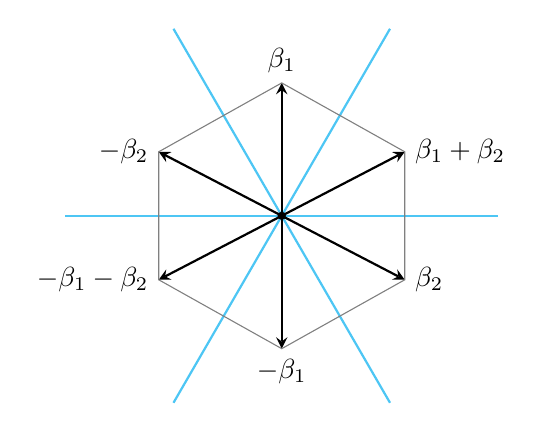
\begin{tikzpicture}[scale=1.25, >=stealth]

            % Hyperplanes
            \draw[cyan!70, thick] (-2.2,0) -- (2.2,0);
            \draw[cyan!70, thick] (-1.1,-1.9) -- (1.1,1.9);
            \draw[cyan!70, thick] (-1.1,1.9) -- (1.1,-1.9);

            % Root vectors
            \draw[->, thick] (0,0) -- (0,1.35) node[above] {\(\beta_1\)};
            \draw[->, thick] (0,0) -- (1.25,0.65) node[right] {\(\beta_1+\beta_2\)};
            \draw[->, thick] (0,0) -- (1.25,-0.65) node[right] {\(\beta_2\)};

            \draw[->, thick] (0,0) -- (0,-1.35) node[below] {\(-\beta_1\)};
            \draw[->, thick] (0,0) -- (-1.25,-0.65) node[left] {\(-\beta_1-\beta_2\)};
            \draw[->, thick] (0,0) -- (-1.25,0.65) node[left] {\(-\beta_2\)};

            % A small hexagon to suggest the root system
            \draw[gray, thin]
            (0,1.35) -- (1.25,0.65) -- (1.25,-0.65) --
            (0,-1.35) -- (-1.25,-0.65) -- (-1.25,0.65) -- cycle;

            % Origin
            \fill (0,0) circle (1.2pt);

        \end{tikzpicture}
    \]
\end{example}

\begin{definition}[Weyl group]
    For \(\alpha\in\Delta\), let \(s_\alpha\) denote the reflection
    \[
        s_\alpha(\lambda)
        =
        \lambda
        -
        \frac{2(\lambda,\alpha)}{(\alpha,\alpha)}\alpha .
    \]
    The subgroup of \(\operatorname{GL}(E)\) generated by all reflections
    \(s_\alpha\), \(\alpha\in\Delta\), is called the \emph{Weyl group} of
    \(\Delta\), and is denoted by
    \[
        W.
    \]
\end{definition}

Since every \(w\in W\) preserves the root system,
\[
    w(\Delta)=\Delta ,
\]
we obtain an injective homomorphism
\[
    W\hookrightarrow \operatorname{Sym}(\Delta).
\]
Hence
\[
    |W|<\infty .
\]

For any base \(B\) of \(\Delta\), denote by
\[
    W_B
    =
    \langle\, s_\beta\mid \beta\in B\,\rangle
\]
the subgroup generated by the simple reflections corresponding to \(B\).

\begin{lemma}
    Let \(B\) be a base of \(\Delta\), and let \(\alpha\in B\). Then
    \(s_\alpha\) permutes the set
    \[
        \Delta^+\setminus\{\alpha\}.
    \]
\end{lemma}

\begin{proof}
    Let
    \[
        \gamma\in \Delta^+\setminus\{\alpha\}.
    \]
    Write
    \[
        \gamma
        =
        \sum_{\beta\in B} k_\beta\beta,
        \qquad
        k_\beta\in\mathbb{Z}_{\geq 0}.
    \]
    Since \(\gamma\neq \alpha\), there exists some \(\beta\in B\), \(\beta\neq\alpha\),
    such that
    \[
        k_\beta>0.
    \]
    Now
    \[
        s_\alpha(\gamma)
        =
        \gamma-\langle \gamma,\alpha^\vee\rangle\alpha,
    \]
    where
    \[
        \langle \gamma,\alpha^\vee\rangle
        =
        \frac{2(\gamma,\alpha)}{(\alpha,\alpha)}
        \in\mathbb{Z}.
    \]
    Thus \(s_\alpha(\gamma)\) has the same coefficients as \(\gamma\) on all
    simple roots \(\beta\neq\alpha\). In particular, the coefficient of the above
    \(\beta\) remains positive.

    Since \(s_\alpha(\gamma)\in\Delta\), it must be either positive or negative
    with respect to the base \(B\). But it cannot be negative, because a negative
    root is a nonpositive integral combination of the simple roots in \(B\), whereas
    \(s_\alpha(\gamma)\) has a positive coefficient on some \(\beta\neq\alpha\).
    Therefore
    \[
        s_\alpha(\gamma)\in\Delta^+.
    \]
    Moreover, \(s_\alpha(\gamma)\neq\alpha\), since otherwise
    \[
        \gamma=s_\alpha(\alpha)=-\alpha,
    \]
    contradicting \(\gamma\in\Delta^+\). Hence
    \[
        s_\alpha(\gamma)\in \Delta^+\setminus\{\alpha\}.
    \]

    Since \(s_\alpha^2=1\), the map \(s_\alpha\) is an involution. Therefore it
    permutes \(\Delta^+\setminus\{\alpha\}\).
\end{proof}

Let \(\Delta\) be a root system in a Euclidean space \(E\), and let \(B\) be
a base of \(\Delta\). Denote by \(\Delta^+=\Delta^+(B)\) the corresponding
set of positive roots, and put
\[
    \rho=\frac12\sum_{\alpha\in\Delta^+}\alpha .
\]
Recall that, for \(\beta\in B\),
\[
    s_\beta(\rho)=\rho-\beta .
\]
Indeed, \(s_\beta\) sends \(\beta\) to \(-\beta\) and permutes
\(\Delta^+\setminus\{\beta\}\).

\begin{lemma}
    Given any two bases \(B\) and \(B'\) of \(\Delta\), there exists
    \(w\in W_B\) such that
    \[
        w(B')=B,
    \]
    where
    \[
        W_B=\langle s_\beta\mid \beta\in B\rangle .
    \]
\end{lemma}

\begin{proof}
    Choose a regular vector \(\gamma'\in E\) corresponding to the base \(B'\),
    so that
    \[
        (\beta',\gamma')>0
        \qquad\text{for all } \beta'\in B'.
    \]
    We want to find \(w\in W_B\) such that
    \[
        (\beta,w(\gamma'))>0
        \qquad\text{for all } \beta\in B.
    \]

    Since \(W_B\) is finite, we may choose \(w\in W_B\) such that
    \[
        (\rho,w(\gamma'))
    \]
    is maximal among all values
    \[
        (\rho,u(\gamma')),
        \qquad u\in W_B.
    \]
    Let \(\beta\in B\). Since \(s_\beta w\in W_B\), the maximality of \(w\)
    gives
    \[
        (\rho,s_\beta w(\gamma'))
        \leq
        (\rho,w(\gamma')).
    \]
    Because \(s_\beta\) is an orthogonal reflection, we have
    \[
        (\rho,s_\beta w(\gamma'))
        =
        (s_\beta\rho,w(\gamma')).
    \]
    Using \(s_\beta(\rho)=\rho-\beta\), we obtain
    \[
        (\rho-\beta,w(\gamma'))
        \leq
        (\rho,w(\gamma')).
    \]
    Hence
    \[
        (\beta,w(\gamma'))\geq 0.
    \]

    In fact, the inequality is strict. If
    \[
        (\beta,w(\gamma'))=0,
    \]
    then
    \[
        (w^{-1}\beta,\gamma')=0.
    \]
    But \(w^{-1}\beta\in\Delta\), while \(\gamma'\) is regular, a contradiction.
    Therefore
    \[
        (\beta,w(\gamma'))>0
        \qquad\text{for all } \beta\in B.
    \]
    Thus \(w(\gamma')\) lies in the Weyl chamber corresponding to \(B\).

    On the other hand, the base corresponding to \(w(\gamma')\) is \(w(B')\).
    Therefore
    \[
        w(B')=B.
    \]
\end{proof}

\begin{lemma}
    Every root \(\alpha\in\Delta\) is contained in some base of \(\Delta\).
\end{lemma}

\begin{proof}
    Let \(\alpha\in\Delta\). Consider the hyperplane
    \[
        \alpha^\perp
        =
        \{x\in E\mid (x,\alpha)=0\}.
    \]
    For every \(\beta\in\Delta\setminus\{\pm\alpha\}\), the subspace
    \[
        \alpha^\perp\cap\beta^\perp
    \]
    is a proper subspace of \(\alpha^\perp\). Since \(\Delta\) is finite and
    \(\alpha^\perp\) cannot be a finite union of proper subspaces, we may choose
    \[
        \rho\in\alpha^\perp
    \]
    such that
    \[
        \rho\notin \beta^\perp
        \qquad
        \text{for all } \beta\in\Delta\setminus\{\pm\alpha\}.
    \]
    Thus
    \[
        (\rho,\beta)\neq 0
        \qquad
        \text{for all } \beta\in\Delta\setminus\{\pm\alpha\}.
    \]

    Now choose a regular vector \(\rho'\) sufficiently close to \(\rho\) such that
    \[
        (\rho',\alpha)>0
    \]
    and
    \[
        |(\rho',\alpha)|
        <
        |(\rho',\beta)|
        \qquad
        \text{for all } \beta\in\Delta\setminus\{\pm\alpha\}.
    \]
    Let \(B_{\rho'}\) be the base corresponding to the regular vector \(\rho'\).
    Then \(\alpha\) is positive with respect to \(B_{\rho'}\).

    We claim that \(\alpha\in B_{\rho'}\). Suppose not. Then \(\alpha\) is a
    positive root which is not simple. Hence there exists a simple root
    \(\beta\in B_{\rho'}\) such that
    \[
        \alpha-\beta\in\Delta^+.
    \]
    Therefore
    \[
        (\rho',\alpha)
        =
        (\rho',\beta)+(\rho',\alpha-\beta),
    \]
    where both terms on the right are positive. Since
    \[
        \beta\neq \pm\alpha,
    \]
    our choice of \(\rho'\) gives
    \[
        (\rho',\beta)
        >
        (\rho',\alpha),
    \]
    which is impossible. Hence \(\alpha\in B_{\rho'}\).

    Therefore every root is contained in some base.
\end{proof}

\begin{corollary}
    For any base \(B\) of \(\Delta\),
    \[
        \Delta=W_B B.
    \]
    Equivalently, every root of \(\Delta\) is \(W_B\)-conjugate to a simple root
    in \(B\).
\end{corollary}

\begin{proof}
    Let \(\alpha\in\Delta\). By the preceding lemma, there exists a base \(B_1\)
    such that
    \[
        \alpha\in B_1.
    \]
    By the first lemma, there exists \(w\in W_B\) such that
    \[
        w(B_1)=B.
    \]
    Hence
    \[
        w(\alpha)\in B.
    \]
    Therefore
    \[
        \alpha\in W_B B.
    \]
    Thus
    \[
        \Delta=W_B B.
    \]
\end{proof}

\begin{corollary}
    For any base \(B\) of \(\Delta\),
    \[
        W=W_B.
    \]
\end{corollary}

\begin{proof}
    By definition,
    \[
        W_B\subseteq W.
    \]
    It remains to prove the reverse inclusion.

    Let \(\alpha\in\Delta\). By the preceding corollary, there exist
    \(w\in W_B\) and \(\beta\in B\) such that
    \[
        w(\alpha)=\beta.
    \]
    Using the conjugation formula for reflections,
    \[
        s_{w(\alpha)}
        =
        w s_\alpha w^{-1},
    \]
    we get
    \[
        s_\beta
        =
        w s_\alpha w^{-1}.
    \]
    Hence
    \[
        s_\alpha
        =
        w^{-1}s_\beta w.
    \]
    Since \(w\in W_B\) and \(s_\beta\in W_B\), it follows that
    \[
        s_\alpha\in W_B.
    \]
    Thus every reflection \(s_\alpha\), \(\alpha\in\Delta\), lies in \(W_B\).
    Since \(W\) is generated by all such reflections, we obtain
    \[
        W\subseteq W_B.
    \]
    Therefore
    \[
        W=W_B.
    \]
\end{proof}

\begin{example}[Irreducible root systems of rank \(2\)]
    Up to isomorphism, the irreducible root systems of rank \(2\) are of types
    \[
        A_2,\qquad B_2,\qquad G_2 .
    \]
    They may be represented by two simple roots whose angles and relative
    lengths are as follows.

    \[
        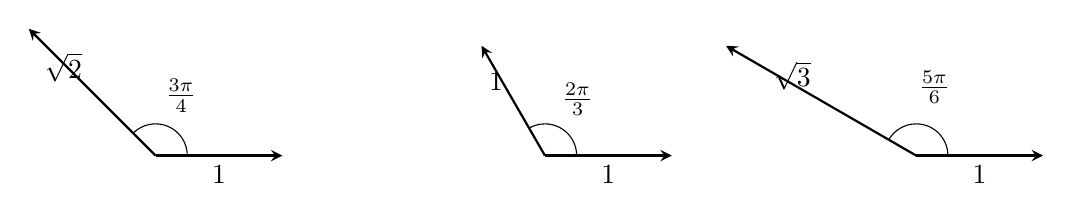
\begin{tikzpicture}[scale=1.15, >=stealth]

            % B2
            \begin{scope}[shift={(0,0)}]
                \coordinate (O) at (0,0);
                \coordinate (a) at (1.4,0);
                \coordinate (b) at ({1.4*sqrt(2)*cos(135)},{1.4*sqrt(2)*sin(135)});

                \draw[->, thick] (O) -- (a) node[midway, below] {\(1\)};
                \draw[->, thick] (O) -- (b) node[midway, above left] {\(\sqrt{2}\)};
                \draw (0.35,0) arc[start angle=0,end angle=135,radius=0.35];
                \node at (67:0.72) {\(\frac{3\pi}{4}\)};
            \end{scope}

            % A2
            \begin{scope}[shift={(4.3,0)}]
                \coordinate (O) at (0,0);
                \coordinate (a) at (1.4,0);
                \coordinate (b) at ({1.4*cos(120)},{1.4*sin(120)});

                \draw[->, thick] (O) -- (a) node[midway, below] {\(1\)};
                \draw[->, thick] (O) -- (b) node[midway, above left] {\(1\)};
                \draw (0.35,0) arc[start angle=0,end angle=120,radius=0.35];
                \node at (60:0.72) {\(\frac{2\pi}{3}\)};
            \end{scope}

            % G2
            \begin{scope}[shift={(8.4,0)}]
                \coordinate (O) at (0,0);
                \coordinate (a) at (1.4,0);
                \coordinate (b) at ({1.4*sqrt(3)*cos(150)},{1.4*sqrt(3)*sin(150)});

                \draw[->, thick] (O) -- (a) node[midway, below] {\(1\)};
                \draw[->, thick] (O) -- (b) node[midway, above left] {\(\sqrt{3}\)};
                \draw (0.35,0) arc[start angle=0,end angle=150,radius=0.35];
                \node at (75:0.78) {\(\frac{5\pi}{6}\)};
            \end{scope}

        \end{tikzpicture}
    \]
\end{example}

\begin{corollary}
    Let \(\alpha,\beta\in\Delta\) be roots with \(\beta\neq\pm\alpha\).
    If \(k\in\mathbb{R}\) and
    \[
        \beta+k\alpha\in\Delta,
    \]
    then
    \[
        k\in\mathbb{Z}.
    \]
\end{corollary}

\begin{proof}
    By the preceding results, \(\alpha\) is contained in some base \(B_1\) of
    \(\Delta\). Write
    \[
        B_1=\{\alpha_1,\alpha_2,\dots,\alpha_\ell\},
        \qquad
        \alpha_1=\alpha .
    \]
    Since \(\beta\in\Delta\), we may write
    \[
        \beta
        =
        \sum_{i=1}^{\ell} k_i\alpha_i,
        \qquad
        k_i\in\mathbb{Z}.
    \]
    Then
    \[
        \beta+k\alpha
        =
        (k_1+k)\alpha_1
        +
        \sum_{i=2}^{\ell} k_i\alpha_i .
    \]
    But \(\beta+k\alpha\in\Delta\). Hence its coordinates with respect to the
    base \(B_1\) are integers. Therefore
    \[
        k_1+k\in\mathbb{Z}.
    \]
    Since \(k_1\in\mathbb{Z}\), it follows that
    \[
        k\in\mathbb{Z}.
    \]
\end{proof}

